\documentclass{article}

\usepackage{graphicx} % to embed images
\usepackage{hyperref} % to link the table of contents

\title{RASD}
\date{2016-11-13}
\author{
	Patricia Abbud
	\and
	Maddalena Andreoli Andreoni
	\and
	Paolo Cudrano
}

\begin{document}
	%%% titlepage %%%
	\begin{titlepage}
		\centering
		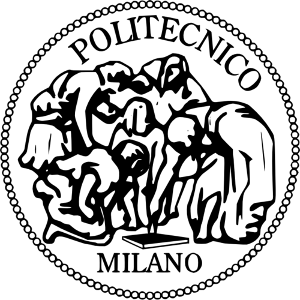
\includegraphics[width=5cm]{img/polimi_logo.png} % also works with logo.pdf
		\vfill
		{\bfseries\Large
			RASD\\
			\vskip4cm
			Patricia Abbud\\
			Maddalena Andreoli Andreoni\\
			Paolo Cudrano\\
		}
		\vfill
		\vfill
	\end{titlepage}

	%%% table of contents %%%
	\tableofcontents
	\newpage

	%%% introduction %%%
	\section{Introduction}
		\subsection{Description of the given problem}
			The system we are going to develop is a car–sharing service called \textit{PowerEnJoy}. The system allows registered users to locate and reserve a car to use.

		\subsection{Goals}
			% this should be adjusted and numbered as soon as everybody has made them
			\begin{itemize}
				%% Pat's part %%
				% TODO

				%% Madda's part %%
				\item \textbf{G1} The system charges the user for a predefined amount of money per minute.
				\item \textbf{G2} The system starts charging the user as soon as the car ignites.
				\item \textbf{G3} The system stops charging the user when the car is parked in a safe area and the user exits the car. The user must confirm the operation, otherwise the system keeps charging them. 
				\item \textbf{G4} A screen on the car notifies the user of the current charges.
				\item \textbf{G5} The system locks the car automatically when the user exits the car. 
				\item \textbf{G6} The system allows the user to open the car through a bluetooth system when the user has reserved it.
				\item \textbf{G8} If the user has chosen to keep being charged, the system allows them to exit and close and re-open the car through a bluetooth system.
				\item \textbf{G9} If the user has chosen to stop being charged, the system keeps a 10–minutes window of time when they are allowed to re-open the car if it has not already been reserved by someone else.
				\item \textbf{G10} The set of safe parking areas is pre–defined by the management system.
				\item \textbf{G11} The system allows the user to earn a 10\% discount on the standard price for the current ride if there are at least two other passengers in the car.

				%% Poe's part %%
				% TODO
			\end{itemize}

		\subsection{Domain properties}
			% TODO
			
			We assume that the following properties hold in the analyzed world:			
			
			% madda's part (kinda -> whatever comes to mind)
			\begin{itemize}
				\item All cars are equipped and located with a GPS system.
				\item All the GPS always give the right position.
				\item The GPS system cannot be switched off.
				\item All cars are equipped with a Bluetooth system.
				\item The Bluetooth system is always on.
				\item The user is always able to be located, either by GPS or by giving their position themselves.
				\item The safe areas are predefined and within the municipality of Milan.
				\item The payment of all services is always accepted. %We're assuming here that the credit card works and has credit, and also that the payment system never breaks. Too much?
				\item The cars always ignite when they are charged %Again, too much? We're assuming the cars never break...
				\item The cars cannot be reserved by more than one user at any given time. %FIXIT move to requirements
				\item The system is always able to tell how many people occupy a car. 
			\end{itemize}

		\subsection{Glossary}
			\begin{description}
				\item[User] We will refer to all people who are registered to the system as 'users'. All users have personal profiles which contain the following information:
				\begin{itemize}
					\item First name;
					\item Family name;
					\item Email;
					\item Username;
					\item Password;
					\item Payment information; this in particular includes
						\begin{itemize}
							\item Credit card number;
							\item Credit card expiration date;
							\item CVV number. %is it called CVV or CCV? I can never remember
						\end{itemize}
					And, optionally:
					\item Personal photo;
					\item Telephone number.
				\end{itemize}
				Users should be able to locate, reserve and drive the cars offered by the service. 
				
				\item[Guest] We shall call 'guests' all people who are using the interface of the system without being registered or logged in. Guests can't access any functionality of \textit{PowerEnJoy} except for the registration process or the log in. 
				
				\item[Safe areas] are predefined parking slots within the municipality.
				\item[Recharging areas] are parking slots where the car can be recharged; safe areas and recharging areas do not always coincide: safe areas \textit{may} be recharging areas, while the contrary doesn't apply. %See and change assumptions whatever we decide.
				
				
				\item[Reservation] We will call 'reservation' the operation of booking a specific car for the sole use of the user who reserved it. Reservations allow the users to access the car, open it and drive it. 
				
				\item[Power grid] %TODO
				
				\item[Standard price] We shall call 'standard price' the price per minute charged to the user, without any discount or sanction applied. 
				
				\item[Discount] A discount always lowers the price per minute charged to a user. It is a negative percentage that is applied every time a user has a virtuous behaviour. 
				\item[Sanction] A sanction always increases the price per minute charged to a user. It is a positive percentage that is applied every time a user has a wasteful or incorrect behaviour. 
				
			\end{description}

		\subsection{Assumptions}
			The assignment document was unclear and ambiguous on some points of the specifications. Hence, we will make the following assumptions:
			
			\begin{itemize}
				\item Safe/rechargin areas
			\end{itemize}

		\subsection{Constrains}
			% TODO

		\subsection{Proposed system}
			% TODO

		\subsection{Identifying Stakeholders}
			% TODO

		\subsection{Reference documents}
			% TODO

	\newpage
	\section{Actors Identifying}
		% TODO

	\newpage
	\section{Requirements}
		% TODO

	\newpage
	\section{Scenario identifying}
		% TODO

	\newpage
	\section{UML models}
		% TODO

	\newpage
	\section{Alloy modeling}
		% TODO

	\newpage
	%%% appendix %%%
	\section{Appendix}
		\listoffigures
		\listoftables
		
		\subsection{Used tools}
		For this assignment, we used the following tools:
		
		\begin{description}
			\item [LaTeX] The group used LaTeX to structure the final document and to help with versioning.
			\item [Github] We leaned on Github for versioning and coordinating synchronized work.
			\item [Toggl] We used toggl to keep track of work hours.
			\item [Alloy]
		\end{description}
		
		\subsection{Hours of work}

\end{document}
